\begin{figure}[h]
\centering
\subfigure[Integration unendlich dünner Ringe zur Berechnung der Fläche.\label{gamma-fig:ring-integration}]{%
    \begin{minipage}[c][4cm][c]{0.3\textwidth}
        \centering
        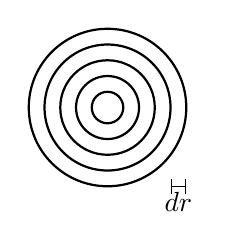
\begin{tikzpicture}
            \foreach \r in {0.2, 0.4, 0.6, 0.8, 1.0} {
                \draw[thick] (0,0) circle (\r cm);
            }
            \draw[{|}-{|}] (0.8,-1) -- (1.0, -1)
                node[midway, yshift=-.2cm] {$dr$};
        \end{tikzpicture}
    \end{minipage}%
}\hfill
\subfigure[Integration unendlich dünner Rechtecke zur Berechnung der Fläche.\label{gamma-fig:rect-integration}]{%
    \begin{minipage}[c][4cm][c]{0.3\textwidth}
        \centering
        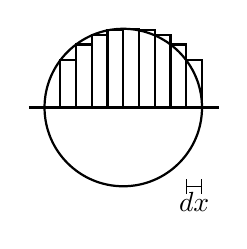
\begin{tikzpicture}
            \def\r{1}
            \draw[{|}-{|}] (0.8,-1) -- (1.0, -1)
                node[midway, yshift=-.2cm] {$dx$};

            \draw[thick] (0,0) circle (\r);
            \draw[thick] (-1.2,0) -- (1.2,0);
            \def\numrect{10}
            \pgfmathsetmacro\dx{2*\r/\numrect}
            \foreach \i in {0,1,...,\numrect} {
                \pgfmathsetmacro\x{-\r + \i*\dx}
                \pgfmathsetmacro\h{sqrt(max(0, \r*\r - \x*\x))}
                \draw[thick] (\x, 0) rectangle ++(\dx, \h);
            }
        \end{tikzpicture}
    \end{minipage}%
}\hfill
\subfigure[Integration von Halbkreisen zur Berechnung des Volumens.\label{gamma-fig:semicircle-integration}]{%
    \begin{minipage}[c][4cm][c]{0.3\textwidth}
        \centering
        \tdplotsetmaincoords{70}{25}
        \begin{tikzpicture}[tdplot_main_coords]
            \def\r{1}
            \def\numrect{8}
            \pgfmathsetmacro\dx{2*\r/\numrect}

            \draw[->] (-\r-0.5, 0, 0) -- (\r+0.5, 0, 0) node[anchor=north east] {$x$};
            \draw[->] (0, -\r-0.5, 0) -- (0, \r+0.5, 0) node[anchor=north west] {$y$};
            \draw[->] (0, 0, -\r-0.5) -- (0, 0, \r+0.5) node[anchor=south] {$z$};

            \foreach \i in {1,...,\numrect} {
                \pgfmathsetmacro\xc{-\r + \i*\dx - 0.5*\dx}
                \pgfmathsetmacro\sliceR{sqrt(max(0, \r*\r - \xc*\xc))}

                \pgfmathsetmacro\nextxc{-\r + (\i+1)*\dx - 0.5*\dx}

                \draw[black, thick, fill=black!10, fill opacity=0.4]
                    plot[domain=0:180, samples=40] ({\xc}, {\sliceR*cos(\x)}, {\sliceR*sin(\x)}) -- cycle;
                \draw[black, thick, fill=black!10, fill opacity=0.4]
                    plot[domain=0:180, samples=40] ({\nextxc}, {\sliceR*cos(\x)}, {\sliceR*sin(\x)}) -- cycle;
                \draw[black, thick] (\xc, \sliceR, 0) -- (\nextxc, \sliceR, 0);
                \draw[black, thick] (\xc, -\sliceR, 0) -- (\nextxc, -\sliceR, 0);
                \draw[black, thick] (\xc, 0.17*\sliceR, \sliceR) -- (\nextxc+0.05,  0.19*\sliceR, \sliceR);
            }

            % \draw[thick, gray] plot[domain=0:360, samples=60] ({\r*cos(\x)}, {\r*sin(\x)}, 0);
            % \draw[thick, gray] plot[domain=0:360, samples=60] ({\r*cos(\x)}, 0, {\r*sin(\x)});
            % \draw[thick, gray] plot[domain=0:360, samples=60] (0, {\r*cos(\x)}, {\r*sin(\x)});

            % dx measurement - aligned with the first slice
            \pgfmathsetmacro\firstX{-\r + 1*\dx - 0.5*\dx}
            \draw[|-|] (\firstX-\dx/2, 0, -\r-0.4) -- (\firstX+\dx/2, 0, -\r-0.4) node[midway, below] {$dx$};
        \end{tikzpicture}
    \end{minipage}%
}
\caption{Intuition hinter Integration über Raum}
\end{figure}
